\section{Results}

\subsection{Community Statistics (? A better title should go here.)}

Discuss the basic properties of the various types of communities: distribution of sizes, number of singletons, etc.

\subsection{Comparing Community-Types with Normalized Mutual Information}

Because OSLOM detects \emph{coverings} rather than \emph{partitions} of users, standard cluster comparison methods like variation of information~\cite{meilua2003comparing} are not appropriate. Instead, we use a generalization of variation of information measure first introduced in~\cite{lancichinetti2009detecting}, the normalized information. \textbf{TK: Etc. Put more here about NMI, what it does, and how to interpret it.}

The normalized mutual information between the various community-types are shown in Figure~\ref{Fig-compare_coverings}. We see that similarity between the coverings is dictated by the generic covering type, with distinct community structure between the structural, activity-based, and interaction-based communities. Interestingly, the communities resulting from the different weightings are all more similar to each other than to the structural communities from the unweighted network.Also note that the communities based on the hashtag similarities are different from both the activity-based and mention-retweet-based communities.

\begin{figure}[h!]
  \centering
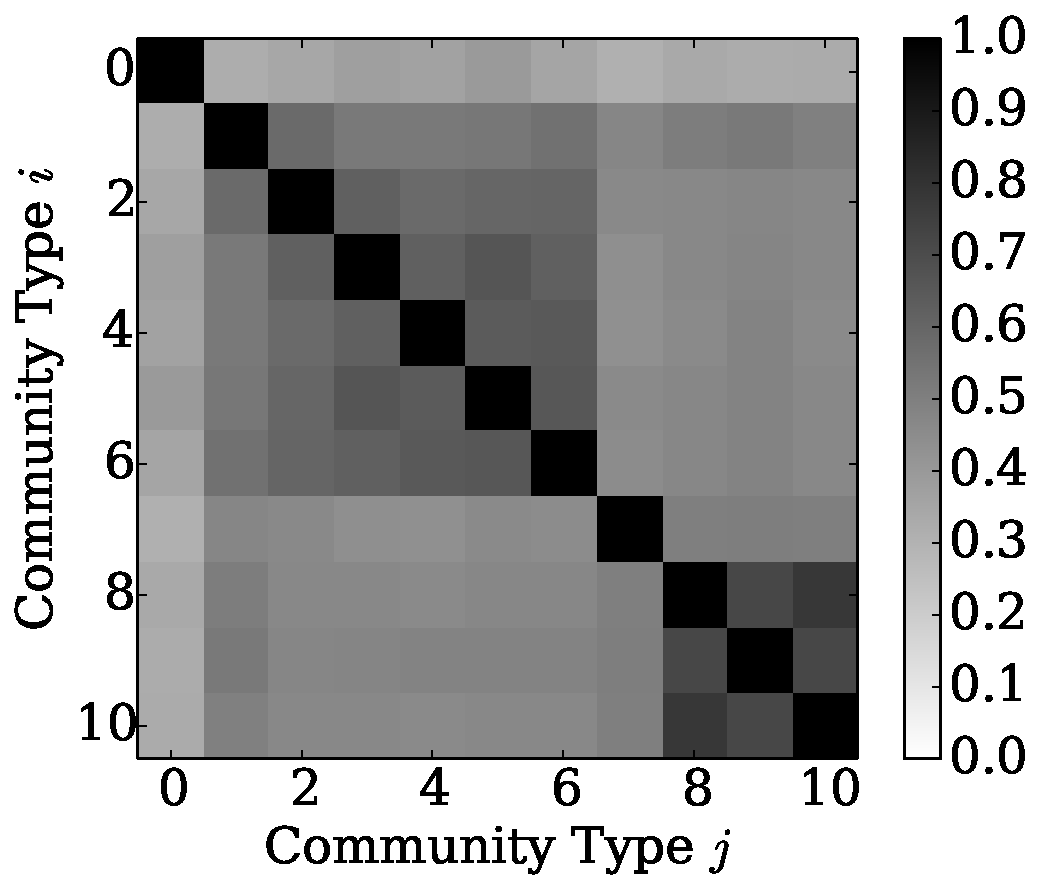
\includegraphics[width=0.50\textwidth]{figures/nmi_singletons.pdf}
\caption{The normalized mutual information between the communities using the different weightings. Weighting 0 corresponds to the structural (binary weighting) network, weightings 1 through 6 correspond to the weighting using the transfer entropy with lag 1 through 6, weighting 7 corresponds to the hashtag similarity, and weightings 8, 9, and 10 correspond to the mention, retweet, and mention-retweet weightings. Values of normalized mutual information close to 1 indicate similarity in the community structure, while values close to 0 indicate dissimilarity. The normalized mutual information is computed with the singletons removed.}
\label{Fig-compare_coverings}
\end{figure}

\subsection{Comparing Different Flows Across Different Community-Types}

\begin{figure}[h!]
  \centering
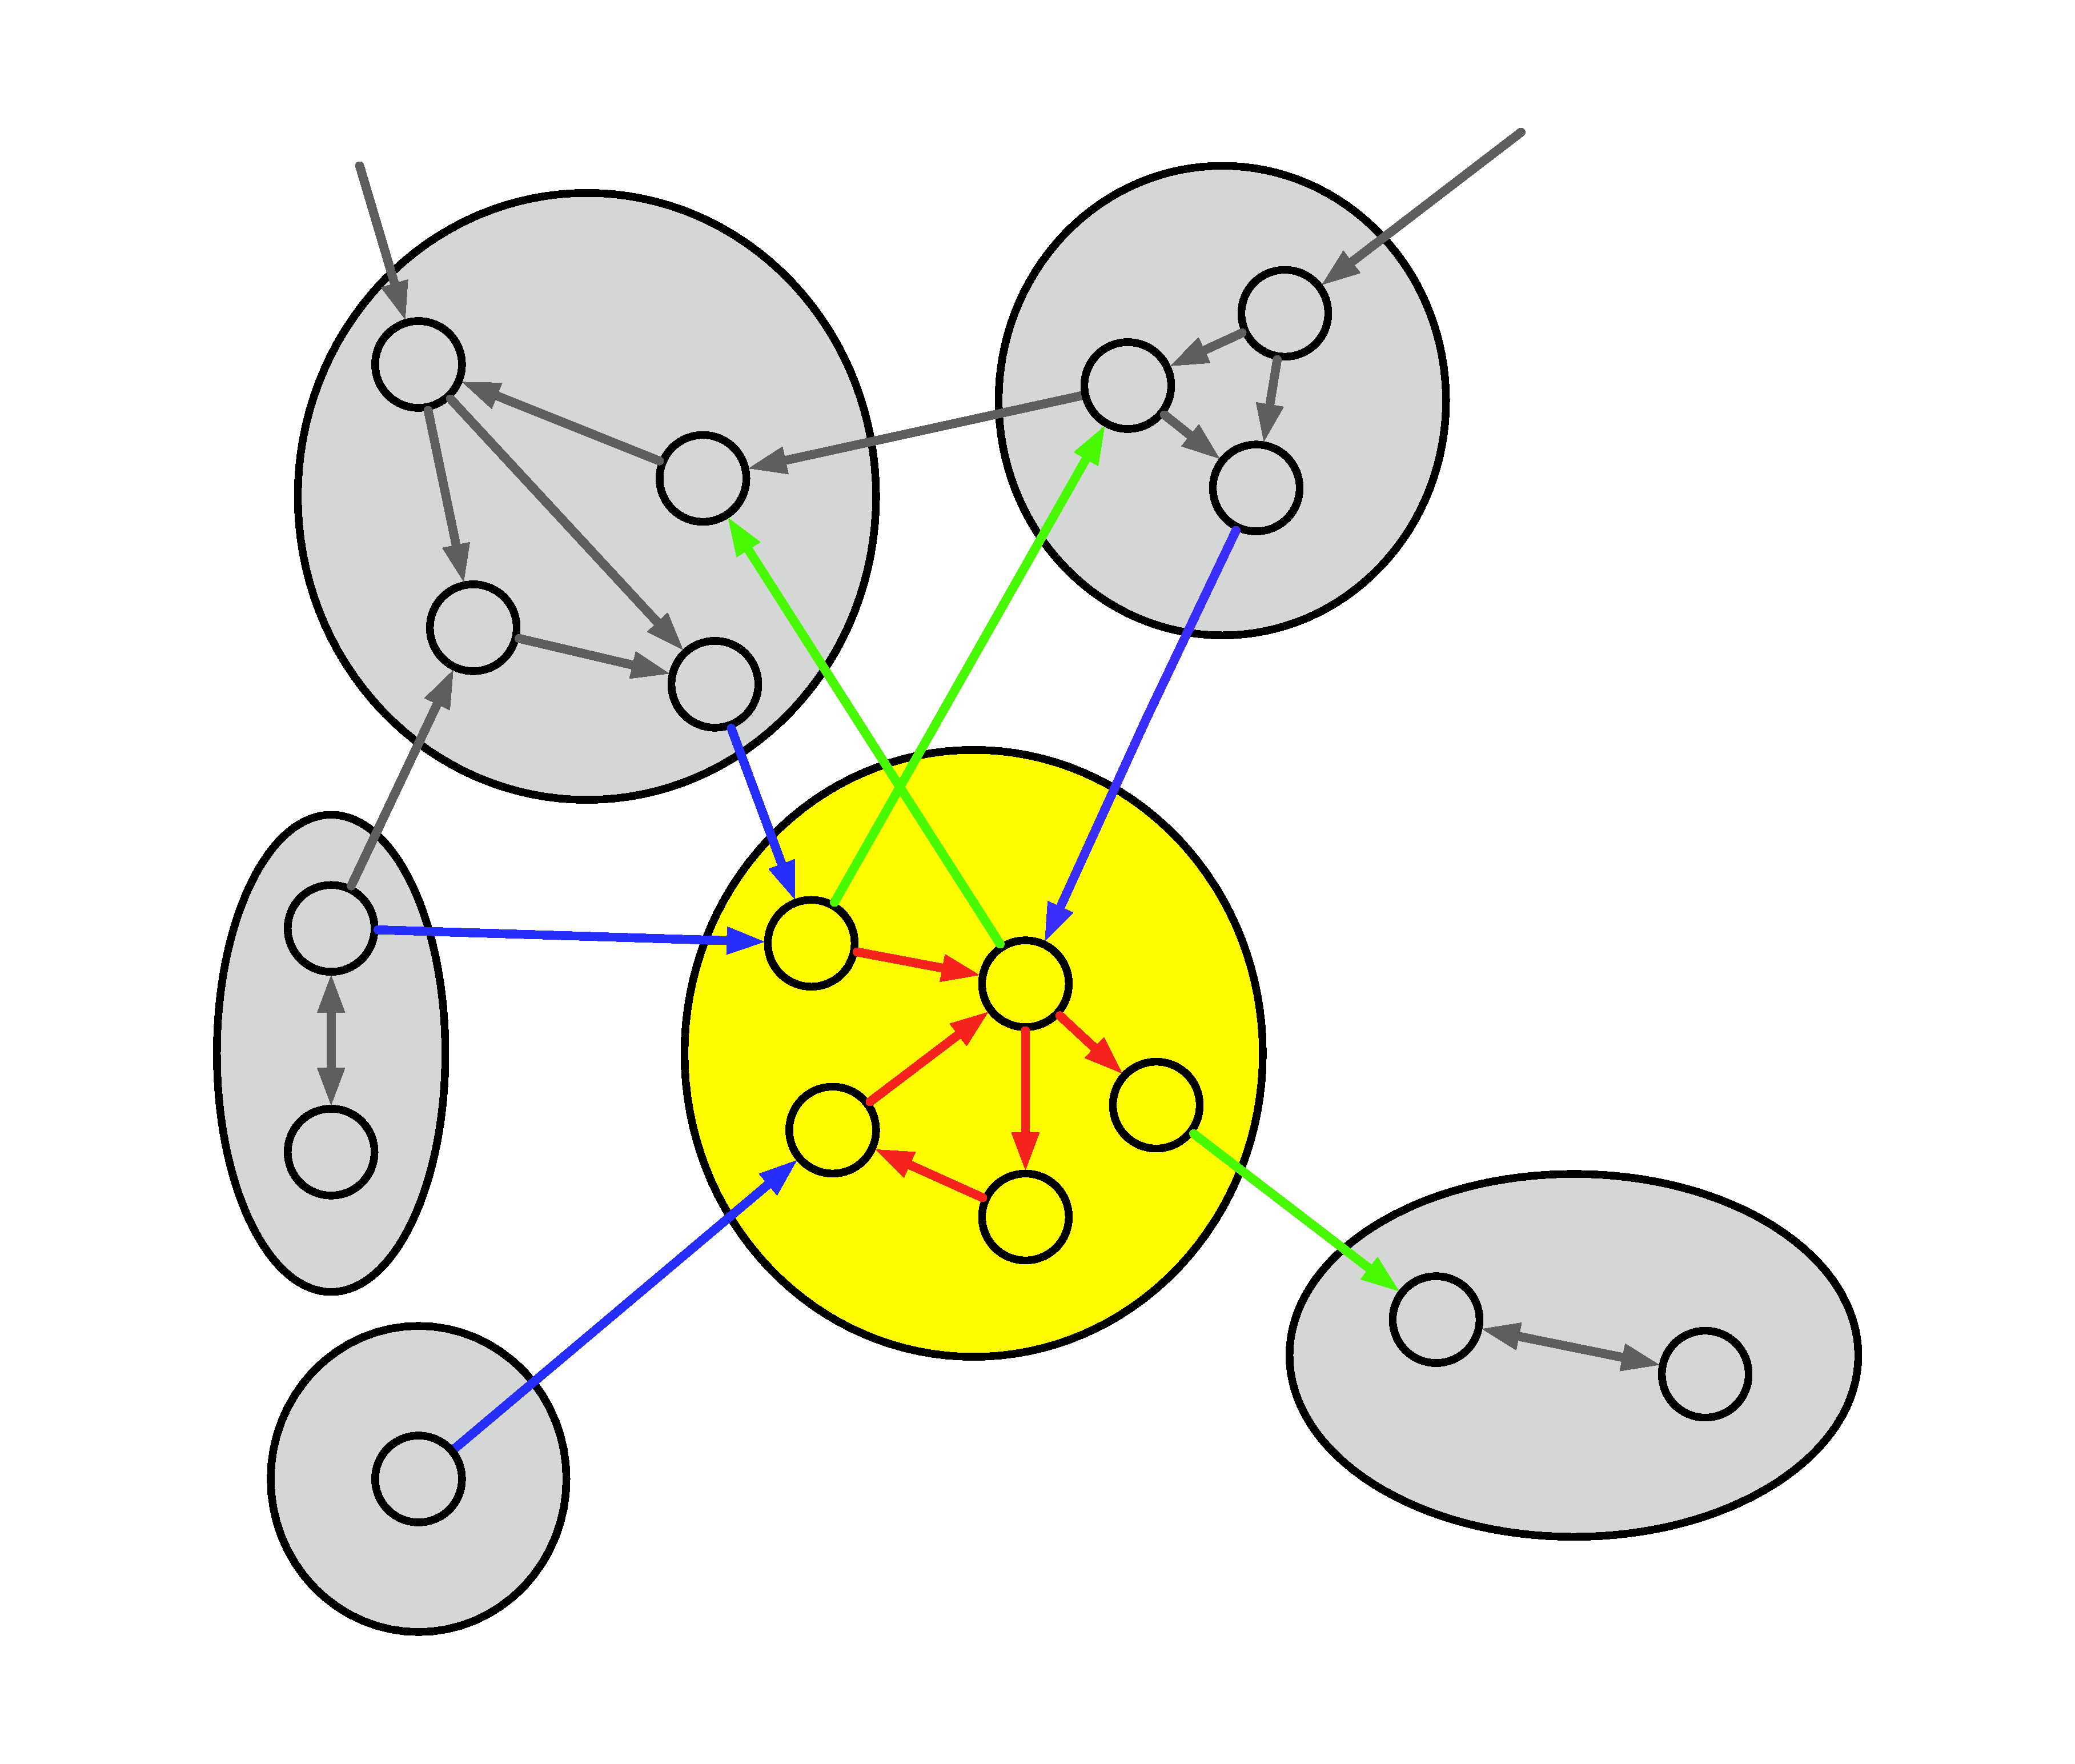
\includegraphics[width=0.50\textwidth]{figures/edge-types.eps}
\caption{An example of the edges considered in determining the edge weight distribution for a given community (the focal community is in yellow). We focus on the internal-to-internal (red), internal-to-external (green), and external-to-internal (blue) edges. For a given focal community, all other edges (grey) are not considered.}
\label{Fig-edge_types}
\end{figure}